\documentclass{../../../oss-ap12ibhl}

\begin{document}
\genheader

\gentitle{11}{ELECTROSTATICS}

\begin{questions}

  \question Two electric objects experience a repulsive force. What happens
  to that force if the distance between the objects is doubled?
  \begin{choices}
    \choice It decreases to one-fourth its value.
    \choice It decreases to one-half its value.
    \choice It stays the same.
    \choice It doubles.
    \choice It quadruples.
  \end{choices}
    
  \question A pith ball is a tiny piece of Styrofoam that is covered with a
  conductive paint. One pith ball initially has a charge of
  \SI{6.4e-8}{\coulomb}, and it touches an identical, neutral pith ball. After
  the pith balls are separated, what is the charge on the pith ball that had
  the initial charge?
  \begin{choices}
    \choice\SI{6.4e-8}{\coulomb}
    \choice\SI{3.2e-8}{\coulomb}
    \choice\SI{0}{\coulomb}
    \choice\SI{-3.2e-8}{\coulomb}
    \choice\SI{-6.4e-8}{\coulomb}
  \end{choices}

  \question Glass becomes positively charged when it is rubbed with silk. Which
  of the following is the best description of what's happening?
  \begin{choices}
    \choice Electrons are rubbed off the glass onto the silk.
    \choice Electrons are rubbed off the silk onto the glass.
    \choice Protons are rubbed off the glass onto the silk.
    \choice Protons are rubbed off the silk onto the glass.
    \choice Neutrons in the glass have an affinity for positive charge.
  \end{choices}

  \question Consider an isolated, neutral system consisting of wool fabric and a
  rubber rod. If the rubber rod is rubbed with wool to become negatively
  charged, what can be said about the wool fabric?
  \begin{choices}
    \choice It becomes equally negatively charged.
    \choice It becomes equally positively charged.
    \choice It becomes negatively charged but not equally.
    \choice It becomes positively charged but not equally.
    \choice In a neutral system, neither object can become charged.
  \end{choices}

  \question An electron and a proton are separated by \SI{1.50e-10}{\metre}. If
  they are released, which one will accelerate at a greater rate, and what is
  the magnitude of that acceleration?
  \begin{choices}
    \choice The electron; \SI{1.12e22}{m/s^2}
    \choice The proton; \SI{1.12e22}{m/s^2}
    \choice The electron; \SI{6.13e18}{m/s^2}
    \choice The proton; \SI{6.13e18}{m/s^2}
    \choice They both accelerate at the same rate; \SI{1.02e-8}{m/s^2}
  \end{choices}

  \question A negatively charged object is placed near, but not touching, a
  neutral conductor. As a result, the two objects are attracted to each other.
  Which of the following is true?
  \begin{choices}
    \choice The neutral object gains positive charges to become positively
    charged.
    \choice The neutral object loses negative charges to become positively
    charged.
    \choice The neutral object loses positive charges to become negatively
    charged.
    \choice The neutral object gains negative charges to become negatively
    charged.
    \choice Negative charges of the neutral object move to the side opposite
    the negatively charged object.
  \end{choices}

  \question A rubber comb is rubbed on hair and then attracts paper bits off the
  table. Which of the following best compares the forces on the paper bits?
  \begin{choices}
    \choice The gravitational force is stronger than the electric force.
    \choice The electric force is stronger than the gravitational force.
    \choice The strong nuclear force dominates all other forces.
    \choice The normal force is stronger than the electric force.
    \choice The magnetic force is stronger than the electric force
  \end{choices}

  \question Which of the following may be said about an object that is a good
  electrical conductor?
  \begin{choices}
    \choice The protons are free to move within the object.
    \choice The electrons are free to move within the object.
    \choice The electrons are bound to their individual atom.
    \choice The object cannot maintain its electric charge.
    \choice It may be made of materials such as rubber and plastic
  \end{choices}
  
  \question Paper is considered an insulator. How does a positively charged
  piece of tape pick up a neutral paper bit?
  \begin{choices}
    \choice The tape makes the protons flow to the opposite end of the paper,
    causing an attraction between the electrons left behind and the tape.
    \choice The tape polarizes the paper atoms, attracting the electrons to the
    side of the atoms closest to the tape.
    \choice The tape forces electrons at the opposite end of the paper to flow
    through the paper toward the tape.
    \choice The tape polarizes the paper atoms, moving the protons within the
    atoms to the side of the atom farthest from the tape.
    \choice It is not possible for a charged object to attract a neutral object.
  \end{choices}
  \vspace{.7in}

  \question Three particles are located on a coordinate system. An electron is
  located at the origin, a proton is located at $(0,1)$, and an electron is
  located at $(1,0)$. What is the direction of the net electrostatic force on
  the electron located at the origin?
  \begin{choices}
    \choice To the right on the coordinate plane
    \choice At an angle of \ang{45} (up and to the right on the coordinate
    plane)
    \choice Up on the coordinate plane
    \choice At an angle of \ang{135} (up and to the left on the coordinate
    plane)
    \choice To the left on the coordinate plane
  \end{choices}
  \newpage
     
  \question A carbon nucleus has 6 protons. What can be said about the
  electrostatic force between an orbital electron and the carbon nucleus?
  \begin{choices}
    \choice The attractive force of the nucleus on the electron is greater than
    the force of the electron on the nucleus.
    \choice The attractive force of the nucleus on the electron is less than the
    force of the electron on the nucleus.
    \choice The attractive force of the nucleus on the electron is equal to the
    force of the electron on the nucleus.
    \choice The repulsive force of the nucleus on the electron is equal to the
    force of the electron on the nucleus.
    \choice The repulsive force of the nucleus on the electron is greater than
    the force of the electron on the nucleus.
  \end{choices}
  \vspace{.7in}
    
  \question A hydrogen nucleus (charge $+e$) and a beryllium nucleus (charge
  $+4e$) experience a force, $F$. Which of the following expressions may be
  used to solve for the distance between the nuclei?

  \begin{oneparchoices}
    \choice$e\sqrt{\dfrac{5k}F}$\hspace{.3in}
    \choice$2e\sqrt{\dfrac{k}F}$\hspace{.3in}
    \choice$\dfrac{4ke^2}F$\hspace{.3in}
    \choice$6Fe^2$\hspace{.3in}
    \choice$3Fe^2$
  \end{oneparchoices}
  \vspace{.5in}
     
  \question Two electrons exert an electrostatic repulsive force on each other.
  Is it possible to arrange the two electrons so the gravitational attraction
  between them is large enough to cancel out the electric repulsive force?
  \begin{choices}
    \choice  No, the charge of the electrons squared is much larger than the
    mass of the electrons squared.
    \choice No, there is no gravitational force between subatomic particles.
    \choice Yes, reducing the radius between the electrons will increase the
    gravitational force as it is proportional to the inverse of the radius
    squared.
    \choice Yes, increasing the distance between the electrons will reduce the
    electrostatic repulsion until it is equal to the gravitational force.
  \end{choices}
  \vspace{.7in}
    
  \question Four charges are arranged at the corners of a square of side a as
  shown. Which of the following is true of the electric field and the electric
  potential at the center of the square?

  \vspace{.1in}
  \begin{minipage}{.3\linewidth}
    \begin{tikzpicture}[scale=2.3]
      \draw[dashed](0,0)--(1,0)--(1,1) node[midway,right]{$a$}--(0,1)--cycle;
      \draw[fill=black](.5,.5) circle(0.03);
      \draw[fill=white](0,0) circle(0.05) node[below]{$-q$};
      \draw[fill=white](1,0) circle(0.05) node[below]{$+q$};
      \draw[fill=white](0,1) circle(0.05) node[above]{$+q$};
      \draw[fill=white](1,1) circle(0.05) node[above]{$-q$};
    \end{tikzpicture}
  \end{minipage}
  \begin{minipage}{.5\linewidth}
    \begin{tabular}{rcc}
      & \underline{Electric Field} & \underline{Electric Potential}\\
      (A) & zero & zero \\
      (B) & $\dfrac{kQ}{a\sqrt{2}}$ & zero \\
      (C) & $\dfrac{kQ^2}{2a^2}$ &  $\dfrac{kQ}{2a}$\\
      (D) & zero &  $\dfrac{kQ}{\sqrt{2a}}$\\
      (E) & $\dfrac{kQ^2}{2a}$ & $\dfrac{kQ}{a\sqrt{2}}$
    \end{tabular}
  \end{minipage}
    
  \question Three charges, $+Q$, $-Q$, and $+2Q$, are arranged in an
  equilateral triangle as shown. Which of the arrows below best represents the
  direction of the electric field at the center of the triangle?

  \begin{minipage}{.3\linewidth}
    \begin{tikzpicture}[scale=2.2]
      \draw[dashed](0,0)--(1,0)--(.5,.866)--cycle;
      \draw[fill=black](.5,.289) circle(.03);
      \draw[fill=white](0,0) circle(.05) node[left]{$+Q\;$};
      \draw[fill=white](1,0) circle(.05) node[right]{$\;-Q$};
      \draw[fill=white](.5,.866) circle(.05) node[above]{$2Q$};
    \end{tikzpicture}
  \end{minipage}
  \begin{minipage}{.6\linewidth}
    \begin{oneparchoices}
      \choice {\huge$\downarrow$}
      \choice {\huge$\uparrow$}
      \choice {\huge$\searrow$}
      \choice {\huge$\swarrow$}
      \choice {\huge$\nearrow$}
    \end{oneparchoices}
  \end{minipage}
  \vspace{.25in}
  
  \question Which of the following diagrams best represents how you might
  rearrange the charges so that the electric field at the center would point
  directly toward the top of the page?

  \begin{oneparchoices}
    \choice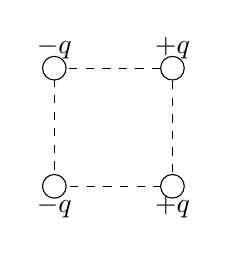
\begin{tikzpicture}[scale=1.5]
      \draw[dashed](0,0) rectangle(1,1);
      \draw[fill=white](0,0) circle(.1) node[below]{$-q$};
      \draw[fill=white](1,0) circle(.1) node[below]{$+q$};
      \draw[fill=white](0,1) circle(.1) node[above]{$-q$};
      \draw[fill=white](1,1) circle(.1) node[above]{$+q$};
    \end{tikzpicture}
    \choice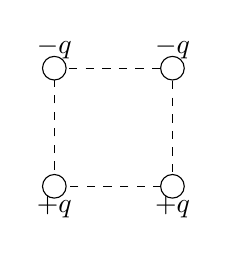
\begin{tikzpicture}[scale=1.5]
      \draw[dashed](0,0) rectangle(1,1);
      \draw[fill=white](0,0) circle(.1) node[below]{$+q$};
      \draw[fill=white](1,0) circle(.1) node[below]{$+q$};
      \draw[fill=white](0,1) circle(.1) node[above]{$-q$};
      \draw[fill=white](1,1) circle(.1) node[above]{$-q$};
    \end{tikzpicture}
    \choice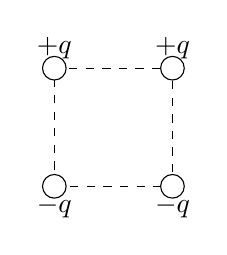
\begin{tikzpicture}[scale=1.5]
      \draw[dashed](0,0) rectangle(1,1);
      \draw[fill=white](0,0) circle(.1) node[below]{$-q$};
      \draw[fill=white](1,0) circle(.1) node[below]{$-q$};
      \draw[fill=white](0,1) circle(.1) node[above]{$+q$};
      \draw[fill=white](1,1) circle(.1) node[above]{$+q$};
    \end{tikzpicture}
    \choice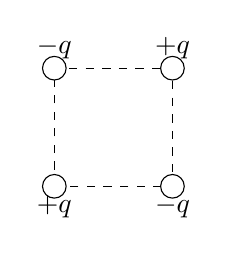
\begin{tikzpicture}[scale=1.5]
      \draw[dashed](0,0) rectangle(1,1);
      \draw[fill=white](0,0) circle(.1) node[below]{$+q$};
      \draw[fill=white](1,0) circle(.1) node[below]{$-q$};
      \draw[fill=white](0,1) circle(.1) node[above]{$-q$};
      \draw[fill=white](1,1) circle(.1) node[above]{$+q$};
    \end{tikzpicture}
    \choice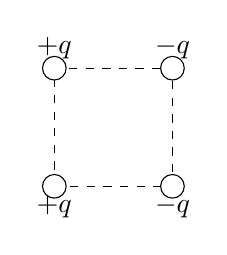
\begin{tikzpicture}[scale=1.5]
      \draw[dashed](0,0) rectangle(1,1);
      \draw[fill=white](0,0) circle(.1) node[below]{$+q$};
      \draw[fill=white](1,0) circle(.1) node[below]{$-q$};
      \draw[fill=white](0,1) circle(.1) node[above]{$+q$};
      \draw[fill=white](1,1) circle(.1) node[above]{$-q$};
    \end{tikzpicture}
  \end{oneparchoices}
  \vspace{.7in}

  \question The electric potential at the surface of the sphere from the last
  question is

  \begin{oneparchoices}
    \choice $\dfrac{\beta R^3}{12\epsilon_0}$\hspace{.2in}
    \choice $\dfrac{\beta R}{2\epsilon_0}$\hspace{.2in}
    \choice $\dfrac{\beta R^3}{3\epsilon_0}$\hspace{.2in}
    \choice $\dfrac{\beta R^2}{2\epsilon_0}$\hspace{.2in}
    \choice $\dfrac{\beta R^2}{4\epsilon_0}$
  \end{oneparchoices}
  \vspace{.2in}
    
  \question Electric potential
  \begin{choices}
    \choice is a vector quantity that depends on the direction of the electric
    field
    \choice is a scalar quantity that depends on the magnitude and sign of
    charges in the vicinity
    \choice is a scalar quantity that depends on the square of the distance from
    the charges in the vicinity
    \choice is a vector quantity that depends on the sign of the charges in the
    vicinity
    \choice is a vector quantity that must point from high to low potential
  \end{choices}

  \question Which of the following statements is true of electric field and
  equipotential lines?
  \begin{choices}
    \choice The electric field vector always points in the same direction as the
    equipotential lines.
    \choice The electric field always points in the opposite direction of the
    equipotential lines.
    \choice The electric field always points perpendicular to the equipotential
    lines.
    \choice The electric field is always equal to the equipotential lines.
    \choice Equipotential lines always form a circle around electric field
    lines.
  \end{choices}

  % FROM TIPLER
  \uplevel{
    \centering
    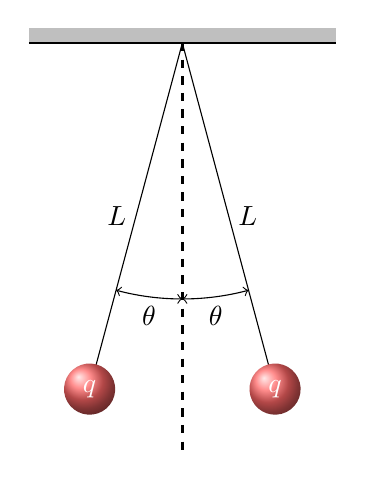
\begin{tikzpicture}[scale=1.3]
      \tikzstyle{balloon}=[ball color=red!60];
      \fill[gray!50](-1.5,0) rectangle(1.5,0.15);
      \draw[thick](-1.5,0)--(1.5,0);
      \draw[dashed,very thick](0,0)--(0,-4);
      \draw[<->](0,-2.5) arc (270:285:2.5) node[midway,below]{$\theta$};
      \draw[<->](0,-2.5) arc (270:255:2.5) node[midway,below]{$\theta$};
      \begin{scope}[rotate=15]
        \draw(0,0)--(0,-3.5) node[midway,right]{$L$};
        \shade[balloon] (0,-3.5) circle (0.25) node[white]{$q$};
      \end{scope}
      \begin{scope}[rotate=-15]
        \draw(0,0)--(0,-3.5) node[midway,left]{$L$};
        \shade[balloon] (0,-3.5) circle (.25) node[white]{$q$};
      \end{scope}
    \end{tikzpicture}
  }
  \question Two identical small spheres of mass $m$ are suspended from a common
  point by threads of length $L$. When each sphere carries a charge $q$, each
  thread makes an angle $\theta$ with the vertical as shown in the figure below.
  \begin{parts}
    \part Express charge $q$ in terms of $\theta$, $m$, $L$ and any other
    relevant constants
    \part Compute $q$ if $m=\SI{10}{\gram}$, $L=\SI{50}{\centi\metre}$ and
    $\theta=\ang{10}$.
  \end{parts}
  \newpage
  
  % FROM TIPLER
  \uplevel{
    \centering
    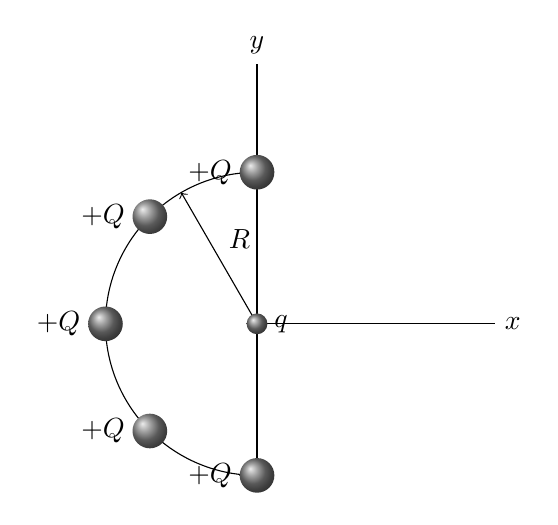
\begin{tikzpicture}[scale=1.1]
      \tikzstyle{balloon}=[ball color=gray];
      \draw(0,-1.75)--(0,3) node[above]{$y$};
      \draw(0,0)--(2.75,0) node[right]{$x$};
      \draw[->,rotate=120](0,0)--(1.75,0) node[midway,above right]{$R$};
      \draw(0,1.75) arc (90:270:1.75);
      \foreach \x in {0,45,...,180}
      \shade[balloon,rotate=\x] (0,1.75) circle(.2) node[left]{$+Q\;\;$};
      \shade[balloon] (0,0) circle(.12) node[right]{$\;q$};
    \end{tikzpicture}
  }
  \question Five equal charges $+Q$ are equally spaced on a semicircle or radius
  $R$ as shown in the figure below. Find the force on a charge $q$ located at
  the center of the semi-circle. (Hint: Take advantage of symmetry.)
  \newpage
  
  % THIS IS TAKEN FROM THE 2001 AP PHYSICS B EXAM FREE-RESPONSE QUESTION #3
  \uplevel{
    \centering
    \begin{tikzpicture}[scale=.8]
      \draw[thick,dashed](0,0)--(4,0) node[midway,below]{$s$}
      --(4,4) node[midway,right]{$s$}--(0,4) node[midway,above]{$s$}
      --(0,0) node[midway,left]{$s$};
      \fill(0,4) circle(.13) node[above left,black]{$+Q$};
      \fill(4,4) circle(.13) node[above right,black]{$-Q$};
      \fill(4,0) circle(.13) node[below right,black]{$+Q$};
      \fill(0,0) circle(.13) node[below right,black]{$-Q$};
    \end{tikzpicture}
    
    Arrangement 1
  }
  
  \question Four charged particles are held fixed at the corners of a square of
  side $s$. All the charges have the same magnitude $Q$, but two are positive
  and two are negative. In Arrangement 1, shown above, charges of the same
  sign are at opposite corners. Express your answers to parts (a) and (b) in
  terms of the given quantities and fundamental constants.
  \begin{parts}
    \part For Arrangement 1, determine the following.
    \begin{subparts}
      \subpart The electric potential at the center of the square
      \subpart The magnitude of the electric field at the center of the square
    \end{subparts}
    \uplevel{
      \begin{center}
        \begin{tikzpicture}[scale=.8]
          \draw[thick,dashed](0,0)--(4,0) node[midway,below]{$s$}
          --(4,4) node[midway,right]{$s$}--(0,4) node[midway,above]{$s$}
          --(0,0) node[midway,left]{$s$};
          \fill(0,4) circle(.13) node[above left,black]{$-Q$};
          \fill(4,4) circle(.13) node[above right,black]{$-Q$};
          \fill(4,0) circle(.13) node[below right,black]{$+Q$};
          \fill(0,0) circle(.13) node[below right,black]{$+Q$};
        \end{tikzpicture}
        
        Arrangement 2
      \end{center}
      The bottom two charged particles are now switched to form Arrangement 2,
      shown above, in which the positively charged particles are on the left and
      the negatively charged particles are on the right.
    }
    
    \part For Arrangement 2, determine the following.
    \begin{subparts}
      \subpart The electrostatic potential at the center of the square
      \subpart The magnitude of the electric field at the center of the square
    \end{subparts}
    
    \part In which of the two arrangements would more work be required to remove
    the particle at the upper right corner from its present position to a
    distance a long way away from the arrangement? Justify your answer.
    
    \vspace{.1in}
    \underline{\hspace{.3in}}Arrangement 1\hspace{.5in}
    \underline{\hspace{.3in}}Arrangement 2
    \vspace{\stretch1}
  \end{parts}
  \newpage

  % THIS IS TAKEN FROM THE 2005 AP PHYSICS B EXAM FREE-RESPONSE QUESTION #3
  \uplevel{
    \centering
    \begin{tikzpicture}
      \draw[thick,->](-5,0)--(5,0)
      node[right]{$x$} node[midway,below left]{$O$};
      \draw[thick,->](0,-3)--(0,3) node[above]{$y$};
      \fill(0,-1.5) circle(.1) node[left]{$-a$} node[right]{$+2q$};
      \fill(0, 1.5) circle(.1) node[left]{$a$}  node[right]{$+q$};
    \end{tikzpicture}
  }
  \question Two point charges are fixed on the y-axis at the locations shown in
  the figure above. A charge of $+q$ is located at $y=+a$ and a charge of $+2q$
  is located at $y=-a$. Express your answers to parts (a) and (b) in terms of
  $q$, $a$, and fundamental constants.
  \begin{parts}
    \part Determine the magnitude and direction of the electric field at the
    origin.
    
    \part Determine the electric potential at the origin.

    \uplevel{
      A third charge of $-q$ is first placed at an arbitrary point $A$
      ($x=-x_0$) on the $x$-axis as shown in the figure below.
      \begin{center}
        \begin{tikzpicture}
          \draw[thick,->](-5,0)--(5,0) node[right]{$x$};
          \draw[thick,->](0,-3)--(0,3) node[above]{$y$};
          \fill(0,-1.5) circle(.1) node[left]{$-a$} node[right]{$+2q$};
          \fill(0, 1.5) circle(.1) node[left]{$a$}  node[right]{$+q$};
          \fill(-4,0)   circle(.1) node[below left]{$A$} node[above]{$-q$};
          \draw[|<->](-4,-.3)--(0,-.3) node[midway,fill=white]{$x_0$};
        \end{tikzpicture}
      \end{center}
    }

    \part Write expressions in terms of $q$, $a$, $x_0$, and fundamental
    constants for the magnitudes of the forces on the $-q$ charge at point $A$
    caused by each of the following.
    \begin{subparts}
      \subpart The $+q$ charge
      \subpart The $+2q$ charge
    \end{subparts}
    
    \part The $-q$ charge can also be placed at other points on the $x$-axis. At
    each of the labeled points ($A$, $B$, and $C$) in the following diagram,
    draw a vector to represent the direction of the net force on the $-q$
    charge due to the other two charges when it is at those points.
    \uplevel{
      \centering
      \begin{tikzpicture}
        \draw[dashed,->](-5,0)--(5,0) node[right]{$x$};
        \draw[dashed,->](0,-3)--(0,3) node[above]{$y$};
        \fill(0,-1.5) circle(.1) node[left]{$-a$} node[right]{$+2q$};
        \fill(0, 1.5) circle(.1) node[left]{$a$}  node[right]{$+q$};
        \fill(-4,0)   circle(.1) node[below]{$A$};
        \fill (0,0)   circle(.1) node[below left]{$B$};
        \fill(2.5,0)  circle(.1) node[below]{$C$};
      \end{tikzpicture}
    }
  \end{parts}
  \newpage

  \uplevel{
    \centering
    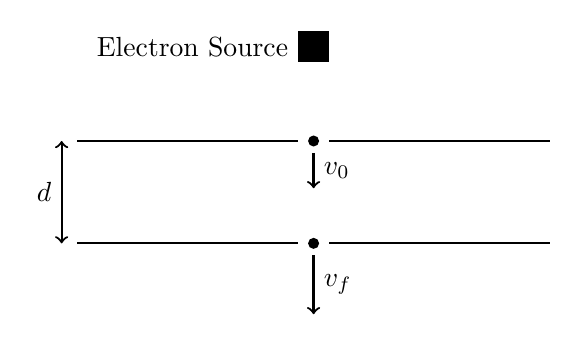
\begin{tikzpicture}
      \fill(-.2,-.2) rectangle(.2,.2);
      \node[left] at (-.2,0){Electron Source};
      \fill(0,-1.2) circle(.07);
      \fill(0,-2.5) circle(.07);
      \draw[thick]( .2,-1.2)--( 3,-1.2);
      \draw[thick](-.2,-1.2)--(-3,-1.2);
      \draw[thick]( .2,-2.5)--( 3,-2.5);
      \draw[thick](-.2,-2.5)--(-3,-2.5);
      \draw[thick,<->](-3.2,-1.2)--(-3.2,-2.5) node[midway,left]{$d$};
      \draw[thick,->](0,-1.35)--(0,-1.8) node[midway,right]{$v_0$};
      \draw[thick,->](0,-2.65)--(0,-3.4) node[midway,right]{$v_f$};
    \end{tikzpicture}

    \underline{Note:} Figure not drawn to scale.
  }
  \question The apparatus shown in the figure above consists of two oppositely
  charged parallel conducting plates, each with area
  $A=\SI{.25}{\metre\squared}$, separated by a distance $d=\SI{.010}{\metre}$.
  Each plate has a hole at its center through which electrons can pass. High
  velocity electrons produced by an electron source enter the top plate with
  speed $v_0=\SI{5.40e6}{\metre\per\second}$, take \SI{1.49}{\nano\second} to
  travel between the plates, and leave the bottom plate with speed
  $v_f=\SI{8.02e6}{\metre\per\second}$.
  \begin{parts}
    \part Which of the plates, top or bottom, is negatively charged? Support
    your answer with a reference to the direction of the electric field between
    the plates.
    
    \part Calculate the magnitude of the electric field between the plates.

    \part Calculate the magnitude of the charge on each plate.

    \part The electrons leave the bottom plate and enter the region inside the
    dashed box shown below, which contains a uniform magnetic field of
    magnitude $B$ that is perpendicular to the page. The electrons then leave
    the magnetic field at point $X$.
    \uplevel{
      \centering
      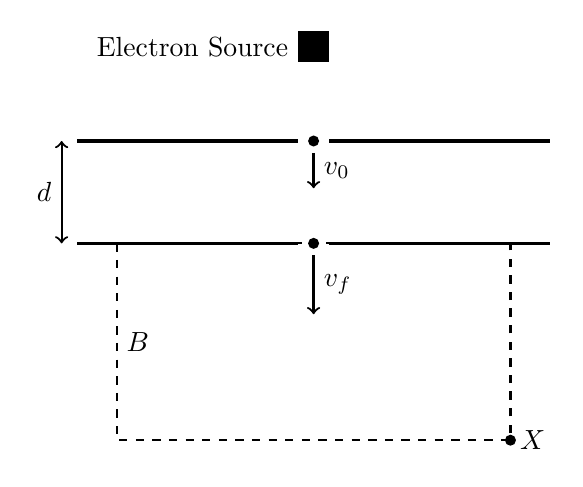
\begin{tikzpicture}
        \fill(-.2,-.2) rectangle(.2,.2);
        \node[left] at (-.2,0){Electron Source};
        \fill(0,-1.2) circle(.07);
        \fill(0,-2.5) circle(.07);
        \draw[very thick]( .2,-1.2)--( 3,-1.2);
        \draw[very thick](-.2,-1.2)--(-3,-1.2);
        \draw[very thick]( .2,-2.5)--( 3,-2.5);
        \draw[very thick](-.2,-2.5)--(-3,-2.5);
        \draw[thick,<->](-3.2,-1.2)--(-3.2,-2.5) node[midway,left]{$d$};
        \draw[thick,->](0,-1.35)--(0,-1.8) node[midway,right]{$v_0$};
        \draw[thick,->](0,-2.65)--(0,-3.4) node[midway,right]{$v_f$};
        \draw[dashed,thick](-2.5,-2.5) rectangle(2.5,-5);
        \node[right] at (-2.5,-3.75){$B$};
        \fill(2.5,-5) circle(.07) node[right]{$X$};
      \end{tikzpicture}

    \underline{Note:} Figure not drawn to scale.
    }
    \begin{subparts}
      \subpart On the figure above, sketch the path of the electrons from the
      bottom plate to point $X$. Explain why the path has the shape that you
      sketched.
      
      \subpart Indicate whether the magnetic field is directed into the page or
      out of the page. Briefly explain your choice.
      \end{subparts}
  \end{parts}
  \newpage

  \uplevel{
    \cpic{.7}{contours}
  }
  \question The dots in the figure above represent two identical spheres,
  $X$ and $Y$, that are fixed in place with their centers in the plane of the
  page. Both spheres are charged, and the charge on sphere $Y$ is positive. The
  lines are isolines of electric potential, also in the plane of the page, with
  a potential difference of \SI{10}{\volt} between each set of adjacent lines.
  The absolute value of the electric potential of the outermost line is
  \SI{50}{\volt}.
  \begin{parts}
    \part Indicate the values of the potentials, including the signs, at the
    labeled points A and B.

    \vspace{.1in}
    Potential at point A \underline{\hspace{.5in}}\hspace{.5in}
    Potential at point B \underline{\hspace{.5in}}

    \part
    \begin{subparts}
      \subpart How do the magnitudes and the signs of the charges of the
      spheres compare? Explain your answer in terms of the isolines of electric
      potential shown.

      \subpart The spheres at points $X$ and $Y$ have masses in the same ratio
      as the magnitudes of their charges. The isolines of gravitational
      potential for the spheres have shapes similar to those of the isolines
      shown. Explain why the two sets of isolines have similar shapes.
    \end{subparts}
    
    \uplevel{
      Let the potentials at the three labeled points be $V_A$, $V_B$, and $V_C$.
      A proton with charge $+q$ and mass $m$ is released from rest at point $B$.
    }
    
    \part Based on your answer to part (b)(ii), briefly describe one similarity
    and one difference between the electric and gravitational forces exerted on
    the proton by the system of the two spheres. The similarity and difference
    you describe must not be ones that generally apply to all forces.
    \newpage
    
    \part At some time after being released from rest at point $B$, the proton
    has moved through a potential difference of magnitude \SI{20}{\volt}.
    \begin{subparts}
      \subpart Determine the change in electric potential energy of the
      proton-spheres system when the proton has moved through the
      \SI{20}{\volt} potential difference. Express your answer symbolically in
      terms of $q$, $V_A$, $V_B$, $V_C$, and physical constants, as appropriate.

      \subpart As it moved through the \SI{20}{\volt} potential difference, the
      proton was displaced a distance d by the electric force. Determine a
      symbolic expression for the total work done on the proton by the electric
      field in terms of the average magnitude E avg of the electric field over
      that distance.

      \subpart Two students are discussing how and why the kinetic energy of
      the proton would change after it is released.
      \begin{itemize}
      \item Student 1 says that if the system is defined as the proton and the
        spheres, the increase in the proton’s kinetic energy is due to a change
        in the system's potential energy as the proton moves through the
        \SI{20}{\volt} potential difference.
      \item Student 2 says that if the system is defined as only the proton,
        the kinetic energy of the proton increases because positive work is
        done on the proton by the electric field as the proton moves through
        the \SI{20}{\volt} potential difference.
      \end{itemize}
      Discuss each student's claims, explaining why each is correct or
      incorrect.
    \end{subparts}
  \end{parts}
\end{questions}
\end{document}
